\chapter{Tracking and Capture System}

\section{Overview}

The tracking and capture system provides the spatial intelligence for our immersive environment, combining sub-millimetre optical tracking for user interaction with cutting-edge volumetric capture for telepresence and analysis.

\section{Optical Motion Tracking System}

\subsection{System Architecture}

\begin{figure}[H]
\centering
\begin{tikzpicture}[scale=0.8]
    % Room outline
    \draw[dreamlabPrimary, ultra thick] (0,0) rectangle (8,6);

    % Tracking cameras in corners
    \foreach \pos in {(0,0), (8,0), (0,6), (8,6)} {
        \draw[fill=dreamlabAccent!30] \pos -- ++(0.6,0.6) -- ++(0,-0.3) -- ++(-0.3,0) -- cycle;
        \draw[fill=black] \pos ++(0.3,0.3) circle (0.1);
    }

    % Additional cameras on walls
    \foreach \x in {4} {
        \draw[fill=dreamlabAccent!30] (\x,0) -- ++(0.3,0.4) -- ++(0.3,0) -- ++(-0.6,0) -- cycle;
        \draw[fill=dreamlabAccent!30] (\x,6) -- ++(0.3,-0.4) -- ++(0.3,0) -- ++(-0.6,0) -- cycle;
    }
    \foreach \y in {3} {
        \draw[fill=dreamlabAccent!30] (0,\y) -- ++(0.4,0.3) -- ++(0,0.3) -- ++(0,-0.6) -- cycle;
        \draw[fill=dreamlabAccent!30] (8,\y) -- ++(-0.4,0.3) -- ++(0,0.3) -- ++(0,-0.6) -- cycle;
    }

    % Tracked users
    \foreach \pos/\label in {(2,2)/1, (5,1.5)/2, (3.5,4)/3, (6,3.5)/4} {
        \draw[fill=dreamlabSecondary!30] \pos circle (0.25);
        \node at \pos {\tiny\label};
        % Tracked markers
        \foreach \angle in {0,120,240} {
            \draw[fill=red] \pos ++(\angle:0.3) circle (0.05);
        }
    }

    \node[below] at (4,-0.5) {\textbf{16-Camera Tracking Configuration}};
\end{tikzpicture}
\caption{Optical tracking camera placement for complete coverage}
\end{figure}

\begin{requirement}{TRK-001}{Minimum 16 high-speed tracking cameras with overlapping coverage}

\begin{requirement}{TRK-002}{Tracking precision <1mm throughout the entire capture volume}

\subsection{Camera Specifications}

\begin{table}[H]
\centering
\begin{tabularx}{\textwidth}{@{}lX@{}}
\toprule
\textbf{Parameter} & \textbf{Specification} \\
\midrule
Camera Model & Vicon Vantage X16 or OptiTrack Prime X 41 \\
Resolution & 16 megapixels (4096 × 4096) \\
Frame Rate & 240Hz standard, 480Hz capability \\
Latency & <3ms from capture to data output \\
IR Illumination & High-power strobed IR LEDs \\
Field of View & 51° × 51° with standard lens \\
Connectivity & 10GigE with PTP synchronisation \\
\bottomrule
\end{tabularx}
\caption{Motion capture camera specifications}
\end{table}

\subsection{Tracking Capabilities}

\begin{itemize}
    \item \textbf{Simultaneous Users}: 6+ with full-body tracking
    \item \textbf{Rigid Bodies}: 20+ tracked objects
    \item \textbf{Individual Markers}: 200+ passive/active markers
    \item \textbf{Capture Volume}: 5m × 5m × 3m minimum
    \item \textbf{Accuracy}: 0.1mm static, 0.5mm dynamic
\end{itemize}

\section{Active Tracking Technology}

\subsection{Active Marker System}

\begin{requirement}{TRK-003}{Active LED markers for robust user identification}

\begin{figure}[H]
\centering
\begin{tikzpicture}[scale=1]
    % Glasses frame
    \draw[thick] (-3,0) -- (-1,0) arc (180:90:0.5) -- (1,0.5) arc (90:0:0.5) -- (3,0);
    \draw[thick] (-3,0) arc (270:180:0.5);
    \draw[thick] (3,0) arc (270:360:0.5);

    % Active markers
    \foreach \pos in {(-2,0.2), (0,0.7), (2,0.2)} {
        \draw[fill=dreamlabSecondary] \pos circle (0.15);
        \draw[dreamlabSecondary, thick] \pos ++(0,0.15) -- ++(0,0.3);
        \draw[dreamlabSecondary, thick] \pos ++(0,0.45) -- ++(0.2,0.1);
        \draw[dreamlabSecondary, thick] \pos ++(0,0.45) -- ++(-0.2,0.1);
    }

    % Sync module
    \draw[fill=dreamlabAccent!30] (-0.5,-0.5) rectangle (0.5,-0.2);
    \node[below] at (0,-0.5) {\tiny Sync};

    \node[below] at (0,-1) {\textbf{Active Tracking Glasses}};
\end{tikzpicture}
\caption{Wireless active marker glasses with unique ID encoding}
\end{figure}

\begin{itemize}
    \item Unique temporal encoding per user (no marker swapping)
    \item Wireless operation with 8+ hour battery life
    \item Integrated shutter sync for stereoscopic viewing
    \item IMU backup for momentary occlusion handling
\end{itemize}

\subsection{Tracked Interaction Devices}

\begin{itemize}
    \item \textbf{Wand Controllers}: 6DOF with buttons and haptic feedback
    \item \textbf{Glove Systems}: Finger-level tracking for gesture input
    \item \textbf{Props}: Custom tracked objects for specific applications
    \item \textbf{Tools}: Tracked stylus for precise 3D annotation
\end{itemize}

\section{Volumetric Capture System}

\subsection{Camera Array Configuration}

\begin{requirement}{TRK-004}{64 synchronised RGB cameras for real-time volumetric capture}

\begin{figure}[H]
\centering
\begin{tikzpicture}[scale=0.6]
    % Room top view
    \draw[dreamlabPrimary, ultra thick] (0,0) rectangle (10,10);

    % Camera positions (simplified representation)
    \foreach \angle in {0,15,...,345} {
        \draw[fill=dreamlabAccent] (5,5) ++(\angle:4.5) circle (0.15);
    }

    % Capture volume
    \draw[dreamlabSecondary, dashed, thick] (5,5) circle (3);

    % Sample coverage lines
    \foreach \angle in {0,45,90,135} {
        \draw[dreamlabDark, opacity=0.3] (5,5) ++(\angle:4.5) -- (5,5);
    }

    \node at (5,5) {\textbf{Capture}};
    \node at (5,4.5) {\textbf{Volume}};

    \node[below] at (5,-0.5) {\textbf{360° Camera Coverage}};
\end{tikzpicture}
\caption{Volumetric capture camera array layout}
\end{figure}

\subsection{Volumetric Camera Specifications}

\begin{table}[H]
\centering
\begin{tabularx}{\textwidth}{@{}lX@{}}
\toprule
\textbf{Parameter} & \textbf{Specification} \\
\midrule
Camera Type & Machine vision global shutter \\
Resolution & 4K (4096 × 2160) minimum \\
Frame Rate & 60fps standard, 120fps capability \\
Sensor & 1" CMOS with high sensitivity \\
Lens & Fixed 8-12mm with remote focus \\
Synchronisation & Hardware genlock to microsecond precision \\
Interface & 10GigE Vision or CameraLink \\
\bottomrule
\end{tabularx}
\end{table}

\section{Volumetric Processing Pipeline}

\subsection{Real-Time Reconstruction}

\begin{requirement}{TRK-005}{Live 3D reconstruction at 30fps with <100ms latency}

\begin{figure}[H]
\centering
\begin{tikzpicture}[scale=0.8]
    % Pipeline stages
    \node[draw, fill=dreamlabPrimary!20] (cap) at (0,0) {Image Capture};
    \node[draw, fill=dreamlabAccent!20] (seg) at (3,0) {Segmentation};
    \node[draw, fill=dreamlabSecondary!20] (depth) at (6,0) {Depth Maps};
    \node[draw, fill=dreamlabPrimary!20] (fusion) at (9,0) {Fusion};
    \node[draw, fill=dreamlabAccent!20] (mesh) at (12,0) {Mesh Output};

    % Connections
    \draw[->, thick] (cap) -- (seg);
    \draw[->, thick] (seg) -- (depth);
    \draw[->, thick] (depth) -- (fusion);
    \draw[->, thick] (fusion) -- (mesh);

    % Timing
    \node[below] at (cap) {\tiny 5ms};
    \node[below] at (seg) {\tiny 15ms};
    \node[below] at (depth) {\tiny 20ms};
    \node[below] at (fusion) {\tiny 30ms};
    \node[below] at (mesh) {\tiny 10ms};

    \node[below] at (6,-1) {\textbf{Total Pipeline: <100ms}};
\end{tikzpicture}
\caption{Volumetric reconstruction pipeline stages}
\end{figure}

\subsection{Processing Infrastructure}

\begin{itemize}
    \item \textbf{Capture Servers}: 8× GPU-accelerated nodes
    \item \textbf{Processing GPUs}: NVIDIA RTX 4090 or better
    \item \textbf{Algorithm}: Neural radiance fields + traditional MVS
    \item \textbf{Output Quality}: 2M polygons at 30fps per person
    \item \textbf{Compression}: Real-time mesh compression for streaming
\end{itemize}

\section{Illumination Systems}

\subsection{Tracking Illumination}

\begin{itemize}
    \item \textbf{IR Flood Lights}: 850nm wavelength
    \item \textbf{Synchronised Strobing}: Matched to camera shutter
    \item \textbf{Intensity Control}: Adaptive based on ambient conditions
    \item \textbf{Safety}: Class 1 eye-safe operation
\end{itemize}

\subsection{Volumetric Capture Lighting}

\begin{requirement}{TRK-006}{Uniform illumination without interfering with display system}

\begin{itemize}
    \item \textbf{White Light Panels}: High-CRI LED arrays
    \item \textbf{Temporal Multiplexing}: Capture during display blanking
    \item \textbf{Colour Temperature}: 5600K daylight balanced
    \item \textbf{Intensity}: 2000 lux at capture volume centre
\end{itemize}

\section{Calibration Systems}

\subsection{Tracking Calibration}

\begin{figure}[H]
\centering
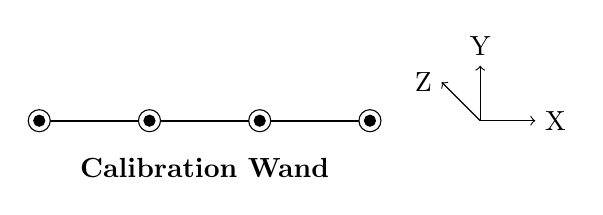
\begin{tikzpicture}[scale=0.7]
    % Calibration wand
    \draw[thick] (0,0) -- (6,0);
    \foreach \x in {0,2,4,6} {
        \draw[fill=white] (\x,0) circle (0.2);
        \draw[fill=black] (\x,0) circle (0.1);
    }
    \node[below] at (3,-0.5) {\textbf{Calibration Wand}};

    % Coordinate system
    \draw[->] (8,0) -- (9,0) node[right] {X};
    \draw[->] (8,0) -- (8,1) node[above] {Y};
    \draw[->] (8,0) -- (7.3,0.7) node[left] {Z};
\end{tikzpicture}
\caption{Precision calibration tools}
\end{figure}

\begin{itemize}
    \item \textbf{Wand Calibration}: Known marker spacing to 0.01mm
    \item \textbf{L-Frame}: Origin and axis definition
    \item \textbf{Volume Accuracy Test}: 27-point validation grid
    \item \textbf{Automated Recalibration}: Weekly schedule
\end{itemize}

\subsection{Volumetric Calibration}

\begin{itemize}
    \item \textbf{Checkerboard Arrays}: Multi-scale pattern detection
    \item \textbf{Bundle Adjustment}: Global optimisation of camera parameters
    \item \textbf{Colour Calibration}: Macbeth chart at multiple positions
    \item \textbf{Geometric Validation}: Tracked object comparison
\end{itemize}

\section{Data Integration and APIs}

\subsection{Tracking Data Protocols}

\begin{requirement}{TRK-007}{Support for industry-standard tracking protocols}

\begin{table}[H]
\centering
\begin{tabularx}{\textwidth}{@{}lX@{}}
\toprule
\textbf{Protocol} & \textbf{Implementation} \\
\midrule
VRPN & Native support with quaternion output \\
OpenXR & Full compliance with tracking extensions \\
OSC & Custom messages for audio spatialisation \\
Unity/Unreal & Direct plugin integration \\
Custom TCP/UDP & Binary protocol for minimum latency \\
\bottomrule
\end{tabularx}
\end{table}

\subsection{Volumetric Data Formats}

\begin{itemize}
    \item \textbf{Live Streaming}: Compressed point clouds via WebRTC
    \item \textbf{Mesh Export}: OBJ, FBX, USD formats
    \item \textbf{Texture Maps}: 4K diffuse, normal, and occlusion
    \item \textbf{Animation}: Alembic cache for temporal sequences
\end{itemize}

\section{Advanced Features}

\subsection{Prediction and Filtering}

\begin{itemize}
    \item \textbf{Kalman Filtering}: Smooth trajectory estimation
    \item \textbf{Predictive Tracking}: 20ms forward prediction
    \item \textbf{Occlusion Handling}: IMU fusion during marker loss
    \item \textbf{Jitter Reduction}: Adaptive smoothing algorithms
\end{itemize}

\subsection{Multi-System Integration}

\begin{requirement}{TRK-008}{Seamless data fusion between tracking and volumetric systems}

\begin{itemize}
    \item Unified coordinate system
    \item Temporal synchronisation to microsecond level
    \item Automatic skeletal tracking from volumetric data
    \item Hybrid tracking for enhanced robustness
\end{itemize}

\section{Performance Metrics}

\subsection{Tracking Performance}

\begin{table}[H]
\centering
\begin{tabularx}{\textwidth}{@{}lXr@{}}
\toprule
\textbf{Metric} & \textbf{Requirement} & \textbf{Target} \\
\midrule
Static Accuracy & <1mm & 0.1mm \\
Dynamic Accuracy & <2mm & 0.5mm \\
Latency & <10ms & 3ms \\
Update Rate & 240Hz & 480Hz \\
Jitter & <0.5mm RMS & 0.1mm RMS \\
\bottomrule
\end{tabularx}
\end{table}

\subsection{Volumetric Performance}

\begin{table}[H]
\centering
\begin{tabularx}{\textwidth}{@{}lXr@{}}
\toprule
\textbf{Metric} & \textbf{Requirement} & \textbf{Target} \\
\midrule
Reconstruction Rate & 30fps & 60fps \\
Geometric Accuracy & <10mm & 5mm \\
Texture Resolution & 4K & 8K \\
Processing Latency & <100ms & 50ms \\
Simultaneous Captures & 2 people & 4 people \\
\bottomrule
\end{tabularx}
\end{table}

\section{Maintenance and Support}

\subsection{Preventive Maintenance}

\begin{itemize}
    \item \textbf{Daily}: System health check via software
    \item \textbf{Weekly}: Lens cleaning and calibration verify
    \item \textbf{Monthly}: Full recalibration procedure
    \item \textbf{Quarterly}: Hardware inspection and testing
\end{itemize}

\subsection{Redundancy and Reliability}

\begin{itemize}
    \item Spare cameras ready for hot-swap
    \item Automatic reconfiguration on camera failure
    \item Redundant processing nodes
    \item Continuous backup of calibration data
\end{itemize}

\begin{center}
\begin{tikzpicture}
\node[rectangle, draw=dreamlabPrimary, fill=dreamlabLight!20, text width=14cm, inner sep=15pt, rounded corners] {
\centering
\textbf{\large\color{dreamlabPrimary}Tracking and Capture Summary}\\[0.5cm]
Our integrated tracking and volumetric capture system provides unprecedented spatial awareness and presence capture. With sub-millimetre optical tracking for interaction and real-time volumetric reconstruction for telepresence, users can naturally interact with virtual content while being captured as photorealistic avatars for remote collaboration.
};
\end{tikzpicture}
\end{center}